\documentclass[11pt]{book}

%%%%%%%%%%%%%%Include Packages%%%%%%%%%%%%%%%%%%%%%%%%%%
\usepackage{xcolor}
\usepackage{mathtools}
\usepackage[a4paper, total={6in, 8in}, margin=1in]{geometry}
\usepackage{amsmath}
\usepackage{amssymb}
\usepackage{paralist}
\usepackage{rsfso}
\usepackage{amsthm}
\usepackage{wasysym}
\usepackage[inline]{enumitem}   
\usepackage{hyperref}
\usepackage{tocloft}
\usepackage{wrapfig}
\usepackage{titlesec}
\usepackage{colortbl}
\usepackage{stackengine} 
\usepackage{csvsimple}
\usepackage{listings}
%%%%%%%%%%%%%%%%%%%%%%%%%%%%%%%%%%%%%%%%%%%%%%%%%%%%%%%%



%%%%%%%%%%%%%%%Code%%%%%%%%%%%%%%%%%%%%%%%%%%%%%%%%%%%%%
\definecolor{codegreen}{rgb}{0,0.6,0}
\definecolor{codegray}{rgb}{0.5,0.5,0.5}
\definecolor{codepurple}{rgb}{0.58,0,0.82}
\definecolor{backcolour}{rgb}{0.95,0.95,0.92}

\lstdefinestyle{mystyle}{
    backgroundcolor=\color{backcolour},   
    commentstyle=\color{codegreen},
    keywordstyle=\color{magenta},
    numberstyle=\tiny\color{codegray},
    stringstyle=\color{codepurple},
    basicstyle=\ttfamily\footnotesize,
    breakatwhitespace=false,         
    breaklines=true,                 
    captionpos=b,                    
    keepspaces=true,                 
    numbers=left,                    
    numbersep=5pt,                  
    showspaces=false,                
    showstringspaces=false,
    showtabs=false,                  
    tabsize=2
}
%%%%%%%%%%%%%%%%%%%%%%%%%%%%%%%%%%%%%%%%%%%%%%%%%%%%%%%%




%%%%%%%%%%%%%%%Chapter Setting%%%%%%%%%%%%%%%%%%%%%%%%%%
\definecolor{gray75}{gray}{0.75}
\newcommand{\hsp}{\hspace{20pt}}
\titleformat{\chapter}[hang]{\Huge\bfseries}{\thechapter\hsp\textcolor{gray75}{$\mid$}\hsp}{0pt}{\Huge\bfseries}
%%%%%%%%%%%%%%%%%%%%%%%%%%%%%%%%%%%%%%%%%%%%%%%%%%%%%%%%

%%%%%%%%%%%%%%%%%Theorem environments%%%%%%%%%%%%%%%%%%%
\newtheoremstyle{break}
  {\topsep}{\topsep}%
  {\itshape}{}%
  {\bfseries}{}%
  {\newline}{}%
\theoremstyle{break}
\theoremstyle{break}
\newtheorem{axiom}{Axiom}
\newtheorem{thm}{Theorem}[section]
\renewcommand{\thethm}{\arabic{section}.\arabic{thm}}
\newtheorem{lem}{Lemma}[thm]
\newtheorem{prop}[lem]{Proposition}
\newtheorem{corL}{Corollary}[lem]
\newtheorem{corT}[lem]{Corollary}
\newtheorem{defn}{Definition}[corL]
\newenvironment{indEnv}[1][Proof]
  {\proof[#1]\leftskip=1cm\rightskip=1cm}
  {\endproof}
%%%%%%%%%%%%%%%%%%%%%%%%%%%%%%%%%%%%%%%%%%%%%%%%%%%%%%


%%%%%%%%%%%%%%%%%%%%%%%Integral%%%%%%%%%%%%%%%%%%%%%%%
\def\upint{\mathchoice%
    {\mkern13mu\overline{\vphantom{\intop}\mkern7mu}\mkern-20mu}%
    {\mkern7mu\overline{\vphantom{\intop}\mkern7mu}\mkern-14mu}%
    {\mkern7mu\overline{\vphantom{\intop}\mkern7mu}\mkern-14mu}%
    {\mkern7mu\overline{\vphantom{\intop}\mkern7mu}\mkern-14mu}%
  \int}
\def\lowint{\mkern3mu\underline{\vphantom{\intop}\mkern7mu}\mkern-10mu\int}
%%%%%%%%%%%%%%%%%%%%%%%%%%%%%%%%%%%%%%%%%%%%%%%%%%%%%%



\newcommand{\R}{\mathbb{R}}
\newcommand{\N}{\mathbb{N}}
\newcommand{\Z}{\mathbb{Z}}
\newcommand{\Q}{\mathbb{Q}}
\newcommand{\C}{\mathbb{C}}
\newcommand{\T}{\mathcal{T}}
\newcommand{\M}{\mathcal{M}}
\newcommand{\Symm}{\text{Symm}}
\newcommand{\Alt}{\text{Alt}}
\newcommand{\Int}{\text{Int}}
\newcommand{\Bd}{\text{Bd}}
\newcommand{\Power}{\mathcal{P}}
\newcommand{\ee}[1]{\cdot 10^{#1}}
\newcommand{\spa}{\text{span}}
\newcommand{\sgn}{\text{sgn}}
\newcommand{\degr}{\text{deg}}
\newcommand{\pd}{\partial}
\newcommand{\that}[1]{\widetilde{#1}}
\newcommand{\lr}[1]{\left(#1\right)}
\newcommand{\vmat}[1]{\begin{vmatrix} #1 \end{vmatrix}}
\newcommand{\bmat}[1]{\begin{bmatrix} #1 \end{bmatrix}}
\newcommand{\pmat}[1]{\begin{pmatrix} #1 \end{pmatrix}}
\newcommand{\rref}{\xrightarrow{\text{row\ reduce}}}
\newcommand{\txtarrow}[1]{\xrightarrow{\text{#1}}}
\newcommand\oast{\stackMath\mathbin{\stackinset{c}{0ex}{c}{0ex}{\ast}{\Circle}}}


\newcommand{\note}{\color{red}Note: \color{black}}
\newcommand{\remark}{\color{blue}Remark: \color{black}}
\newcommand{\example}{\color{green}Example: \color{black}}
\newcommand{\exercise}{\color{green}Exercise: \color{black}}

%%%%%%%%%%%%%%%%%%%%%%Roman Number%%%%%%%%%%%%%%%%%%%%%%%
\makeatletter
\newcommand*{\rom}[1]{\expandafter\@slowromancap\romannumeral #1@}
\makeatother
%%%%%%%%%%%%%%%%%%%%%%%%%%%%%%%%%%%%%%%%%%%%%%%%%%%%%%%%%

%%%%%%%%%%%%table of contents%%%%%%%%%%%%%%%%%%%%%%%%%%%%
\setlength{\cftchapindent}{0em}
\cftsetindents{section}{2em}{3em}

\renewcommand\cfttoctitlefont{\hfill\huge\bfseries}
\renewcommand\cftaftertoctitle{\hfill\mbox{}}

\setcounter{tocdepth}{2}
%%%%%%%%%%%%%%%%%%%%%%%%%%%%%%%%%%%%%%%%%%%%%%%%%%%%%%%%%


%%%%%%%%%%%%%%%%%%%%%Footnotes%%%%%%%%%%%%%%%%%%%%%%%%%%%
\newcommand\blfootnote[1]{%
  \begingroup
  \renewcommand\thefootnote{}\footnote{#1}%
  \addtocounter{footnote}{-1}%
  \endgroup
}
%%%%%%%%%%%%%%%%%%%%%%%%%%%%%%%%%%%%%%%%%%%%%%%%%%%%%%%%%

%%%%%%%%%%%%%%%%%%%%%Section%%%%%%%%%%%%%%%%%%%%%%%%%%%%%
\makeatletter
\def\@seccntformat#1{%
  \expandafter\ifx\csname c@#1\endcsname\c@section\else
  \csname the#1\endcsname\quad
  \fi}
\makeatother
%%%%%%%%%%%%%%%%%%%%%%%%%%%%%%%%%%%%%%%%%%%%%%%%%%%%%%%%%

%%%%%%%%%%%%%%%%%%%%%%%%%%%%%%%%%%%Enumerate%%%%%%%%%%%%%%
\makeatletter
% This command ignores the optional argument 
% for itemize and enumerate lists
\newcommand{\inlineitem}[1][]{%
\ifnum\enit@type=\tw@
    {\descriptionlabel{#1}}
  \hspace{\labelsep}%
\else
  \ifnum\enit@type=\z@
       \refstepcounter{\@listctr}\fi
    \quad\@itemlabel\hspace{\labelsep}%
\fi}
\makeatother
\parindent=0pt
%%%%%%%%%%%%%%%%%%%%%%%%%%%%%%%%%%%%%%%%%%%%%%%%%%%%%%%%%%


\begin{document}

	\begin{titlepage}
		\begin{center}
			\vspace*{1cm}
			\Huge \color{red}
				\textbf{Lab 7 Report}\\
			\vspace{0.5cm}			
			\Large \color{black}
				Math 391 - Introduction to Modern Physics Lab\\
				Professor Wayne Lau\\	
				University of Michigan\\
			\vspace{3cm}

			
\includegraphics[scale=1]{hmm.pdf}\\
			
			
			\vspace{5cm}
			\LARGE
				\textbf{Jinyan Miao}\\
				\hfill\break
				\LARGE Fall 2022\\
			\vspace{1cm}

		\vspace*{\fill}
		\end{center}			
	\end{titlepage}


\newpage
\tableofcontents
\addtocontents{toc}{~\hfill\textbf{Page}\par}


\setcounter{chapter}{6}
\chapter*{Lab 7 - Solar Spectroscopy}
\section{Introduction}
The dark absorption lines in the solar spectrum were first found by William Wollaston in 1802. This feature is mainly due to the processes in the solar photosphere and chromosphere, but might also be caused by molecular oxygen in the Earth's atmosphere. In Lab 7 of Physics 391, we use the Vermier spectrometer to obtain solar spectral measurements and identify some of the absorption lines in the spectrum. Also, in the second part of the lab, we focus particularly on the absorption line for $\text{CO}_2$ and estimate the order of magnitude of the effect of the small amounts of $\text{CO}_2$ in air. \\

\section{Experimental Setup}
For the first part of the lab, we measure the solar spectrum by using Vermier spectrometer. The spectrometer is connected to a computer and operated by the program Logger Pro. Three sample spectra of the Sun are obtained on October 21st, 2022, at Randall Lab. The spectra cover wavelengths from $350\, nm$ to $900\, nm$. The data measurement process is similar to that in Lab 6, where we tune the sample rate to make sure the intensity in the spectra is not oversaturated. We then use Microsoft Excel to analyze the spectra, and the analysis part is discussed in the next section.\\

In the second part of the experiment. The apparatus that we use is a small optical system consisting of an incandescent lamp as a light source and two small sapphire lenses to produce a parallel light beam that is then focused to the surface of an infrared detector with a narrow band filter designed to match the wavelength band corresponding to one of the strong $\text{CO}_2$ molecular absorption lines. The relative intensity of the detector output is displayed. We measure the response of the intensity when the concentration of the $\text{CO}_2$ in the region between the two lenses is changed. We change the concentration in two ways, (1) via human breath, and (2) via the use of a box of soda. A white Delrin matching base is placed between the two lens mounts and $\text{CO}_2$ is made through it. \\
\newpage

\section{Data Analysis}
\subsection{Solar Spectrum}
We analyze our three spectra using Microsoft Excel. The spacing of the sample wavelength in the sample is taken to be around $0.7\, nm$. For each wavelength in the data set, the average of the intensity of the three spectra is computed. We use an algorithm to compute the dip in the spectra. If the intensity $y_i$ for a wavelength satisfies the following condition when comparing with the intensity of nearby wavelengths:
\begin{align}
y_{i-2} > y_{i-1} > y_i \qquad\qquad y_i<y_{i+1} < y_{i+2}
\end{align}
Then the wavelength $\lambda$ approximated by the following is identified as a dip in the spectra:
\begin{align*}
\lambda_{dip} = \frac{\sum_{j=i-2}^{i+2}\lambda_j \cdot (\max\{y_{i-2}, y_{i+2}\}-y_j)}{\sum_{j=i-2}^{i+2}(\max\{y_{i-2},y_{i+2}\}-y_j)}
\end{align*}
The result is depicted in the following figure, with the blue curve representing the spectral intensity for given wavelength, and red indicators indicating the dip of the wavelengths.\\
\begin{center}
\textbf{Figure 1. Solar Spectrum and Absorption Lines}\\
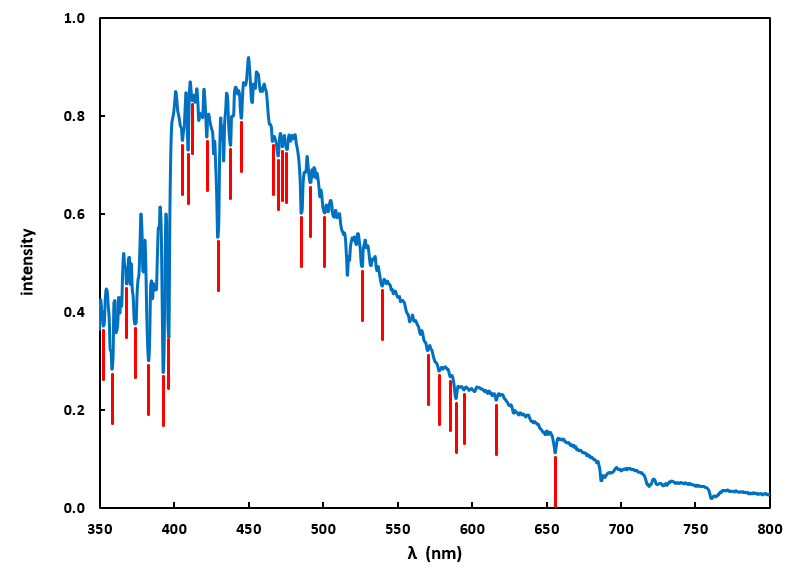
\includegraphics[scale=0.8]{spectral}
\end{center}

We note that some dip in Fig. 1 are not identified by the algorithm. This is due to the fact that the algorithm identify dips strictly following formula (6.1). As a result, if two dips fall in the range within 2 spacing of the sample wavelength, according to (6.1), neither of the two will be identified. For example, the dips around $\lambda = 680\, nm$ and the dips around $\lambda = 760\, nm$ are not identified by the algorithm. Hence one way to improve this experiment is by improving the algorithm to find the dips. One possible way to improve the algorithm is to perform curve fit around the dips that we can physically observed from the diagram, and identify all other dips via (6.1).\\



We identify the dip of intensities with an absorption line according to the database \textit{NIST Atomic Spectra Database Lines Data} [1]. We also computed the relative strength of each dip for comparison. The results are given by the following table:

\begin{center}
\begin{tabular}{|c|c|c|c|c|}%
\hline
     \bfseries Dip $\lambda$ & \bfseries Relative Dip Strength &\bfseries Intensity &\bfseries Expected $\lambda$ & \bfseries Element
    \csvreader[head to column names]{data.csv}{}
    {\\\hline\csvcoli&\csvcolii&\csvcoliii
      &\csvcoliv&\csvcolv}\\% specify your coloumns here
\hline  
\end{tabular}
\end{center}  
On another note, when there are many spectral lines close to the measured wavelength, we identify the most abundant element in the solar photosphere among all possible candidates. On the other hand, the identification process is subjective, and we are not statistically sure that the identification is correct. The
calibration of the spectrometer also generates small random error which might lead to the wrong identification of the absorption lines. We suggest performing the same experiment in different days to get a more robust and statistical identification of the absorption lines. 

\newpage
\subsection{CO$_2$ Absorption}
The measurements are given by the following table:
\begin{center}
\begin{tabular}{|c|c|}
\hline
\textbf{Concentration of CO$_2$} & \textbf{Relative Intensity}\\
\hline
Air & 0.727\\
\hline
Chi Han's breath & 0.120\\
\hline
Soda water & 0.331\\
\hline
\end{tabular}
\end{center}
We see that the reading of the relative intensity on the detector decreases from $0.727$ to $0.120$ as Chi exhales via a tube connected to the region between the lenses, and go back to the air relative intensity when he inhales. Similar changes in the reading is observed for the soda water, from $0.727$ to $0.331$. The observation suggests that a small change in the concentration of CO$_2$ in air leads to a relative huge change in the intensity of some wavelengths in the spectrum. That is, when CO$_2$ blocks some fraction of the blackbody radiation emanating from the surface, the Earth equilibrium temperature will be affected.\\


\subsection{Temperature on Mars Surface}
Here we perform a calculation to approximate the temperature on the Mars' surface. The solar intensity at Mars orbit is given by the following:
\begin{align*}
I = \frac{4\pi R_{sun}^2\sigma T_{sun}^2}{4\pi D^2} = \frac{1361}{1.5^2}\, W/m^2 = 604.889 \, W/m^2
\end{align*}
and hence we write:
\begin{align*}
T_{mars} \approx \sqrt{\frac{\sqrt{1-\text{albedo}}R_{sun}}{2D}}\cdot T_{sum} = \sqrt{\frac{\sqrt{1-\text{0.16}} (6.957\cdot 10^{8}\, m) }{2(224.29\cdot 10^{6}\, m)}}\cdot (5778\, K) = 217.84\,K
\end{align*}
Hence the temperature on the surface of Mars is around $217.84\, K$. \\

\section{Summary}
In Lab 7 of Physics 391, we measure the solar spectrum and approximate the absorption lines by locating the dips in the spectrum. We also estimate the order of magnitude of the effect of small change in the amount of CO$_2$ in air, and calculated the temperature of the Mars surface to be around $217.84\, K$. 

\section{Reference}
\begin{enumerate}
\item Kramida, A., Ralchenko, Yu., Reader, J., and NIST ASD Team (2022). NIST Atomic Spectra Database (ver. 5.10), [Online]. Available: https://physics.nist.gov/asd [2022, November 4]. National Institute of Standards and Technology, Gaithersburg, MD. DOI: https://doi.org/10.18434/T4W30F
\end{enumerate}


\end{document}